\documentclass[12pt,]{article}
\usepackage[T1]{fontenc}
\usepackage[utf8]{inputenc}
\usepackage{fullpage}

% \usepackage{authblk}
\usepackage{graphicx}
\usepackage{subfig}
\graphicspath{{./figures/}}

\usepackage[left]{lineno}
\linenumbers

\title{A comprehensive study of the early phylodynamics of SARS-CoV-2 in Europe}

\begin{document}
\maketitle

\abstract{This project focus on the spatial dynamics of the early spread of SARS-CoV-2 in Europe. We apply a novel approach based on the Multi-type Birth Death phylodynamic model to infer structured population dynamics jointly with between-subpopulation transmission rates from viral genome sequences. The inferred epidemic trajectories for the combined outbreak responsible for the observed sequence data will allow us to better understand the entry into and early spread of SARS-CoV-2 in Europe.}

\section{Results}

\begin{figure}[ht]
    \centering
    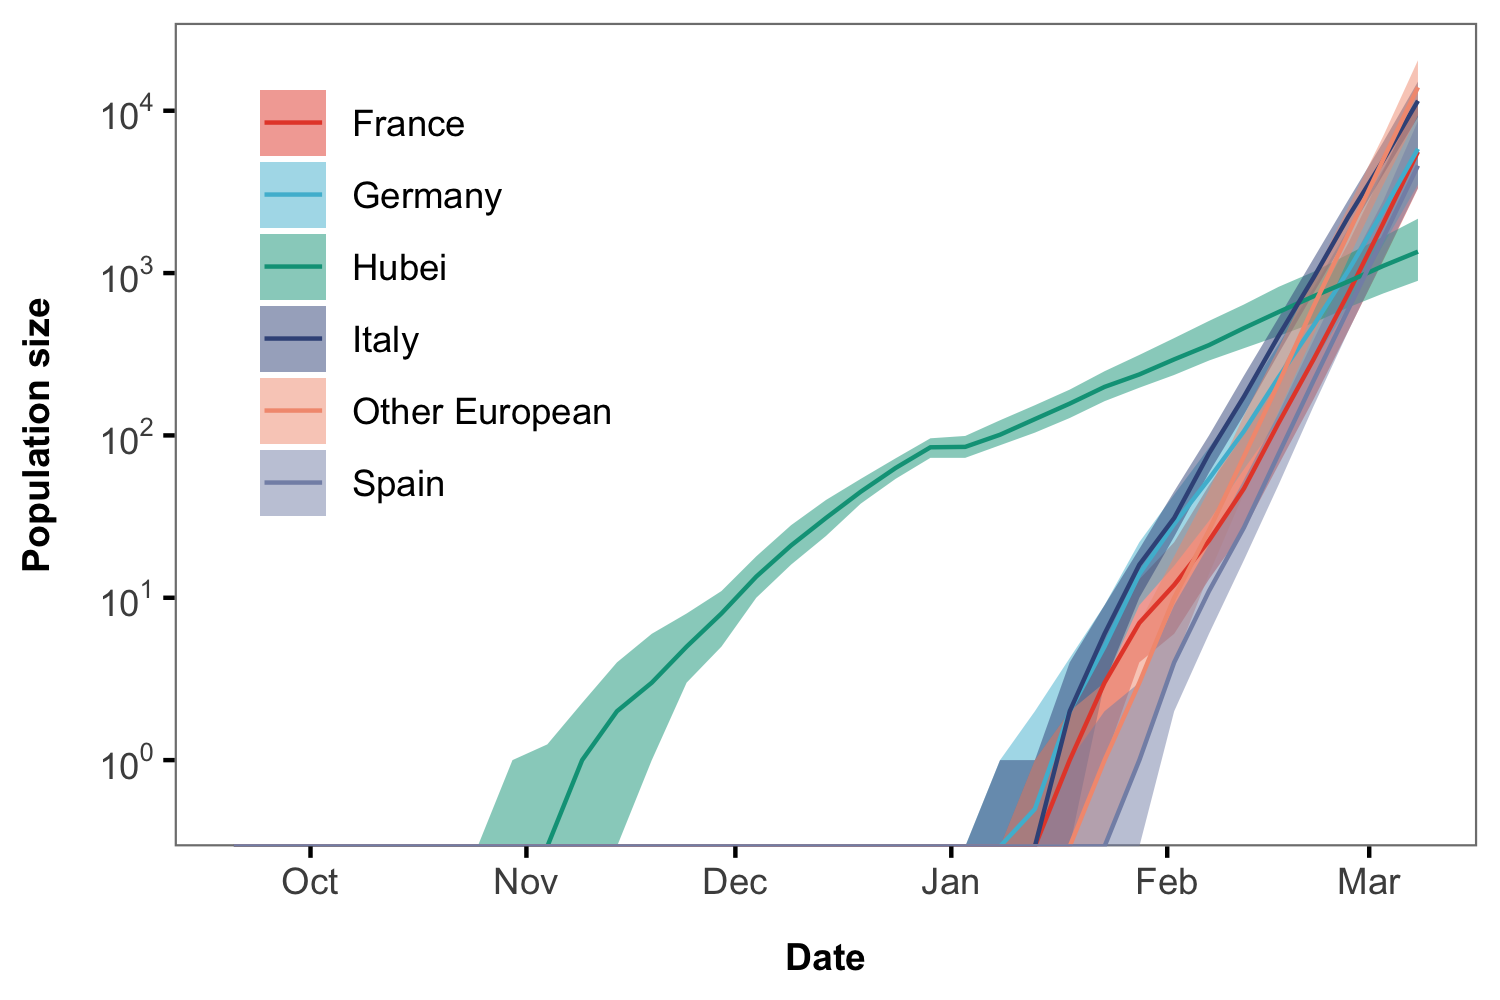
\includegraphics[width=0.8\textwidth]{201014_europe2_figtraj01.png}
    \caption{Inferred population size summary statistics for each deme over time. The line represents the median population trajectory and the interval is the interquartile range from a subsampled set of inferred population trajectories. Color represents the different demes in the analysis.}
    \label{fig:gribbon}
\end{figure}

\begin{figure}[ht]
    \centering
    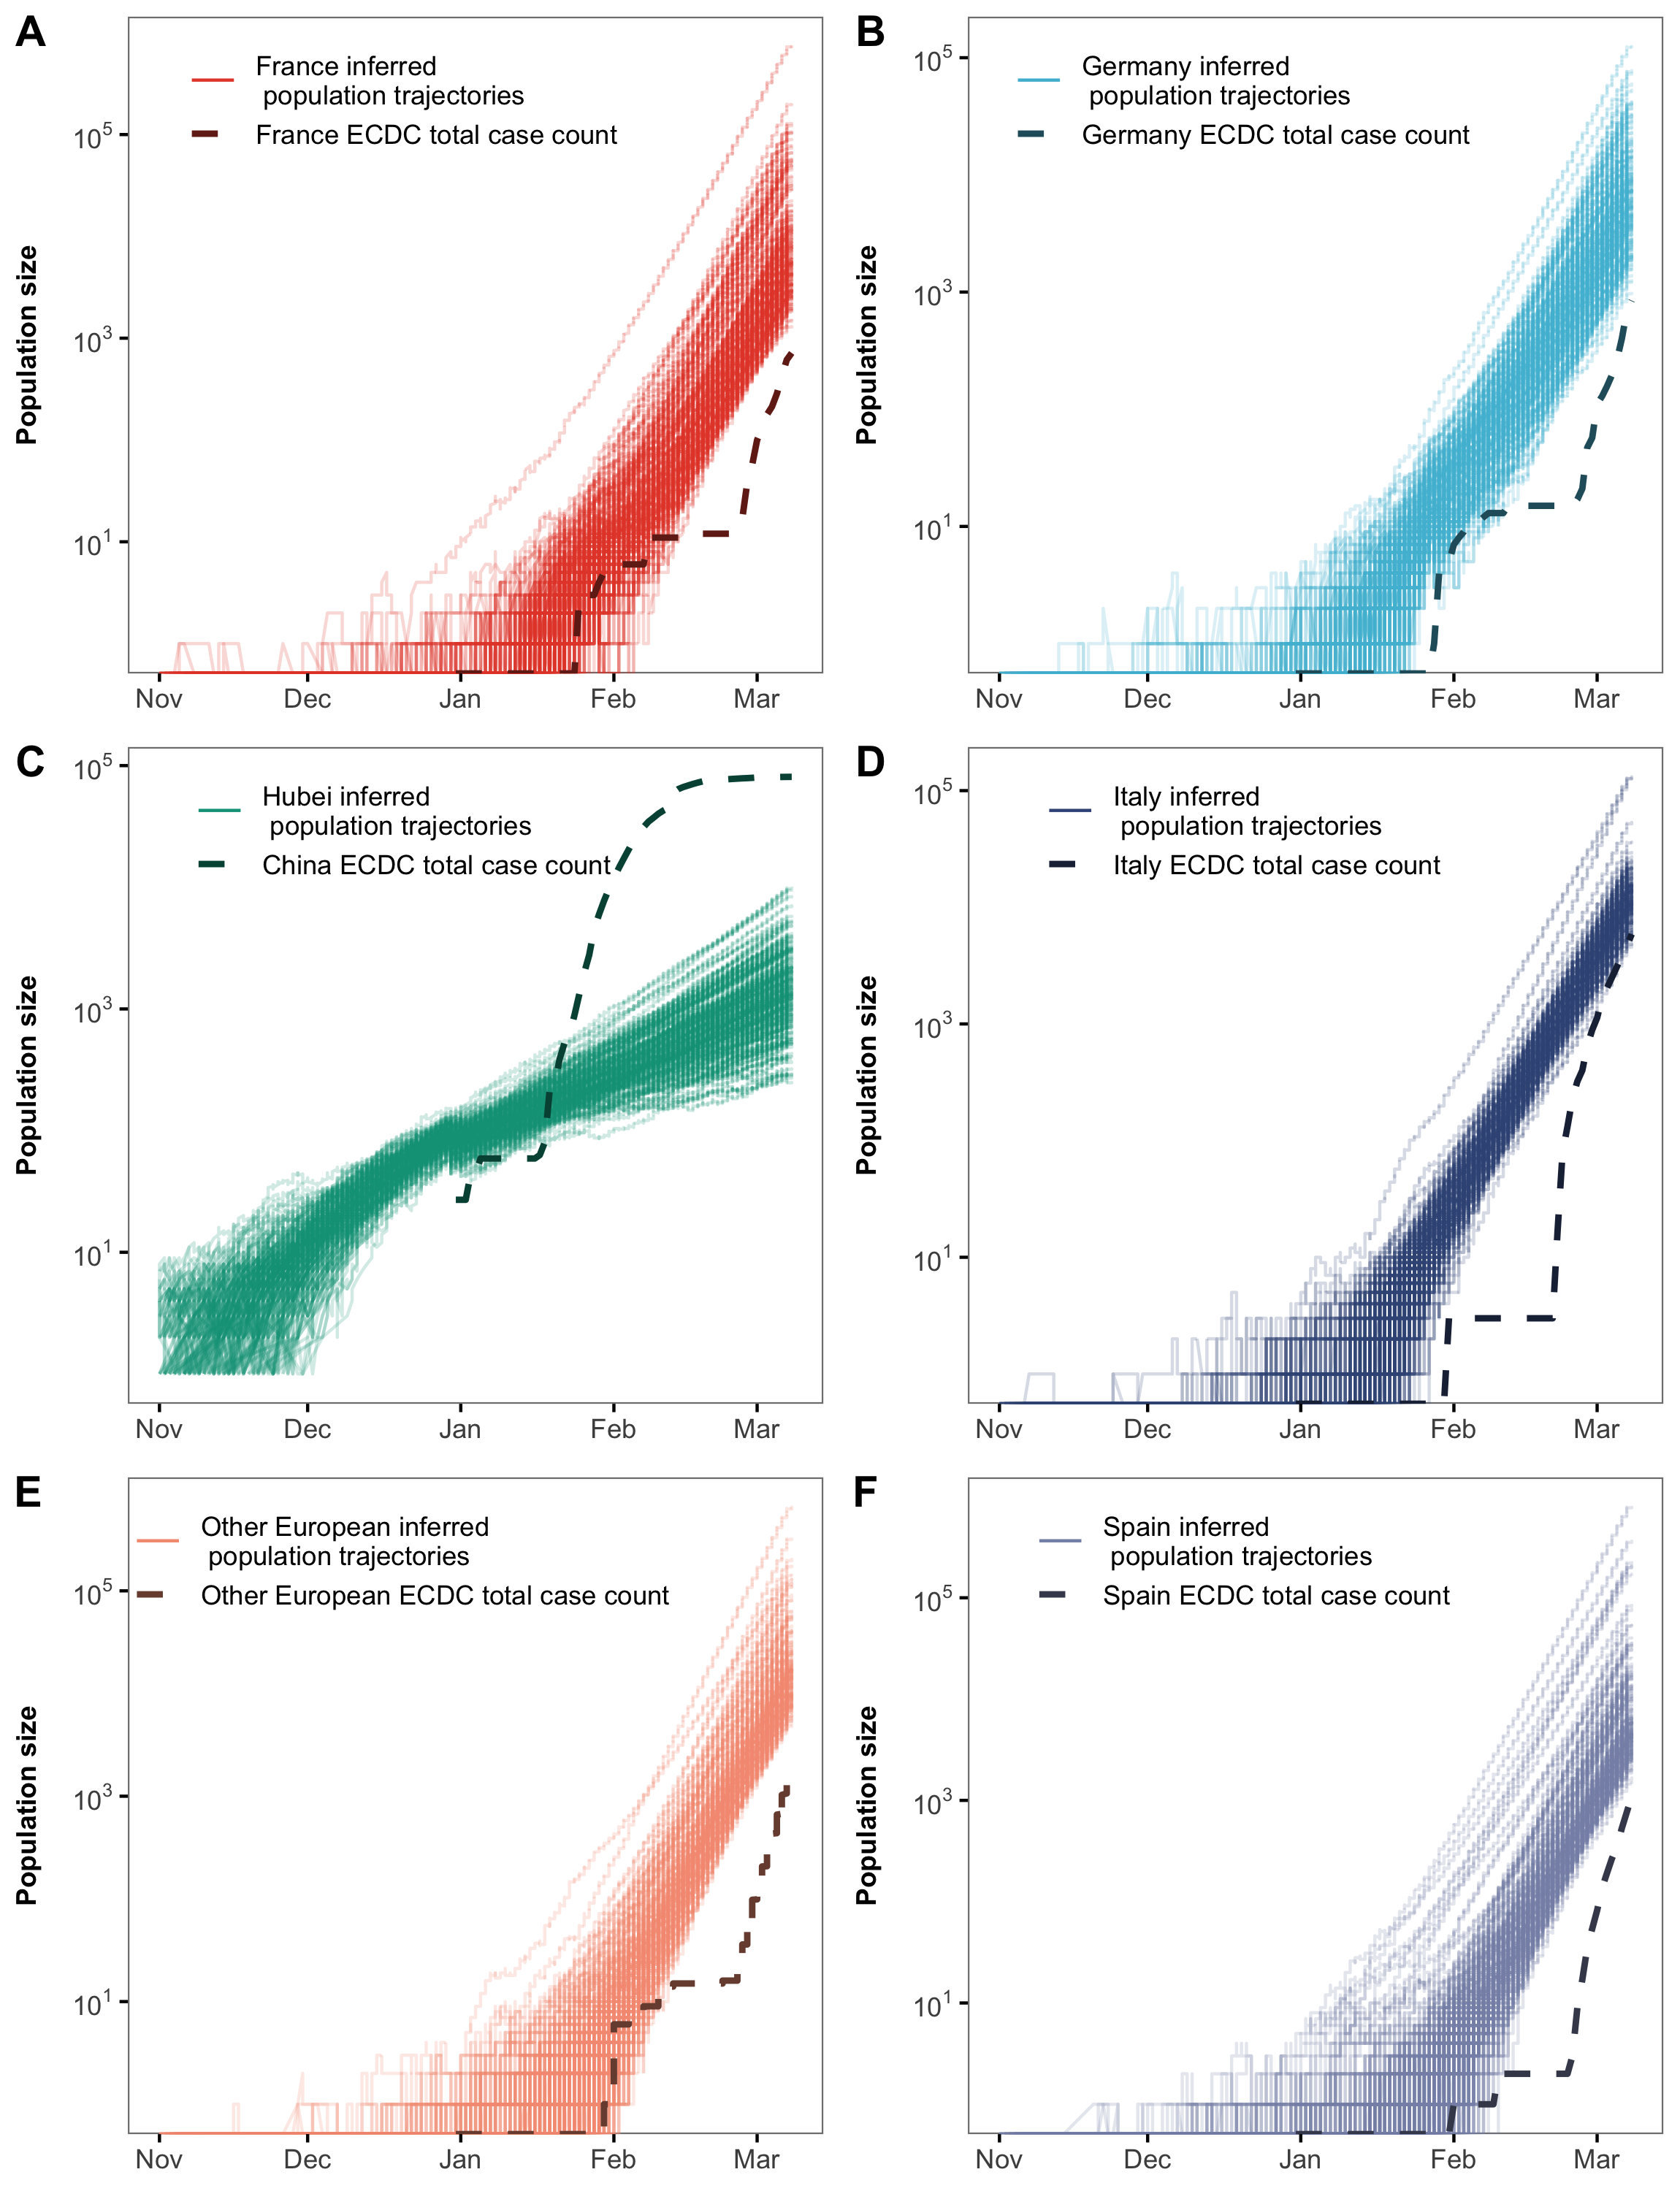
\includegraphics[width=0.9\textwidth]{201014_europe2_figtraj02.png}
    \caption{Inferred population size trajectories over time. A subsampled set of 200 inferred trajectories is plotted. In each subplot, the trajectories (solid lines) are compared with the ECDC total case count data (dashed line).}
    \label{fig:trajs}
\end{figure}

\begin{figure}[!tbp]
  \centering
  \subfloat[Temporal distribution of first introduction.]{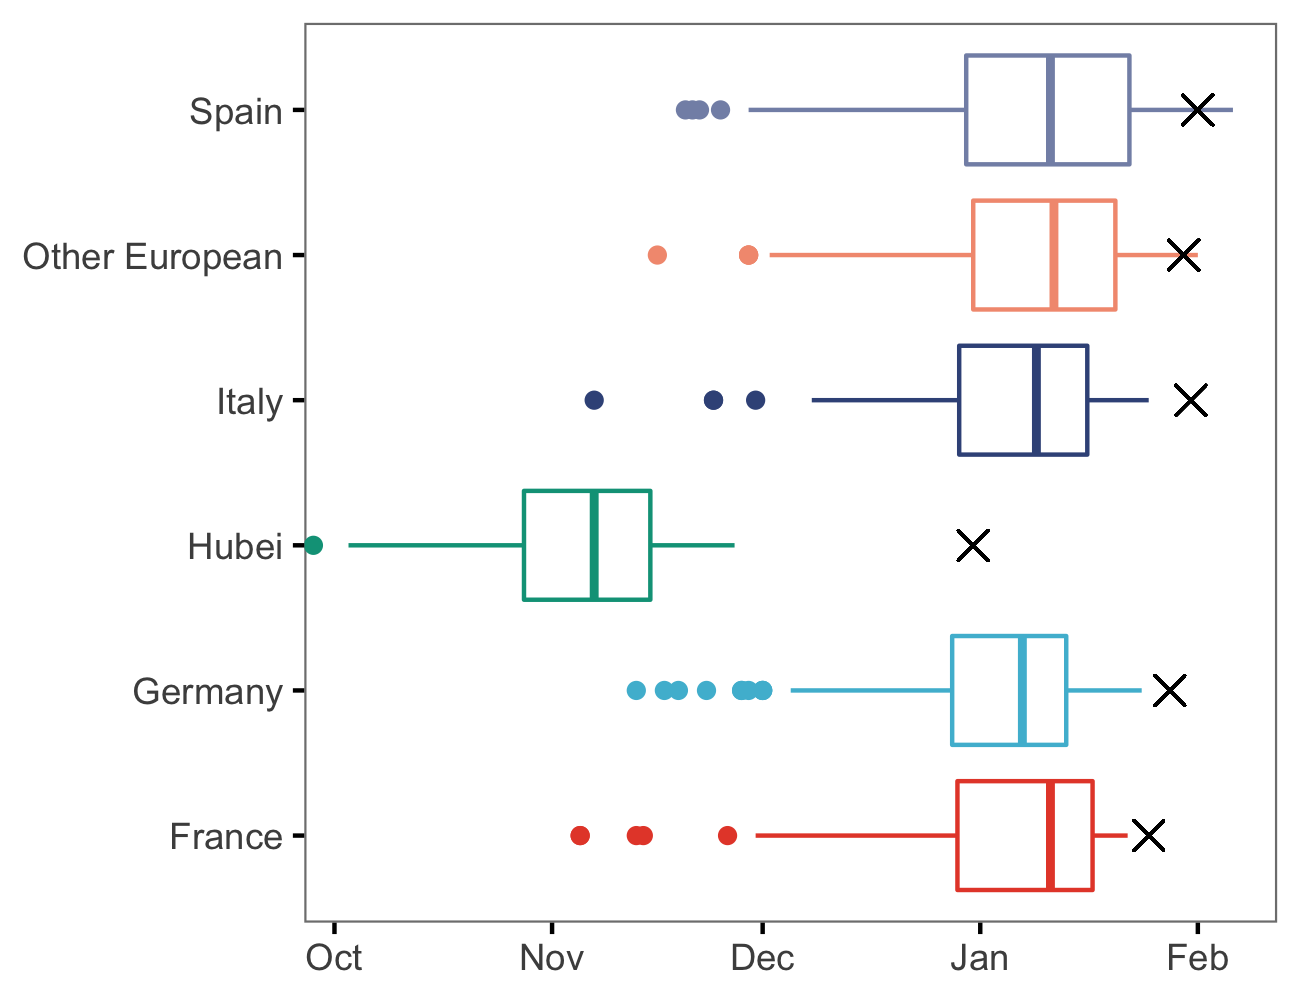
\includegraphics[width=0.5\textwidth]{201014_europe2_figtraj03.png}\label{fig:f1}}
  \subfloat[Source of first introduction.]{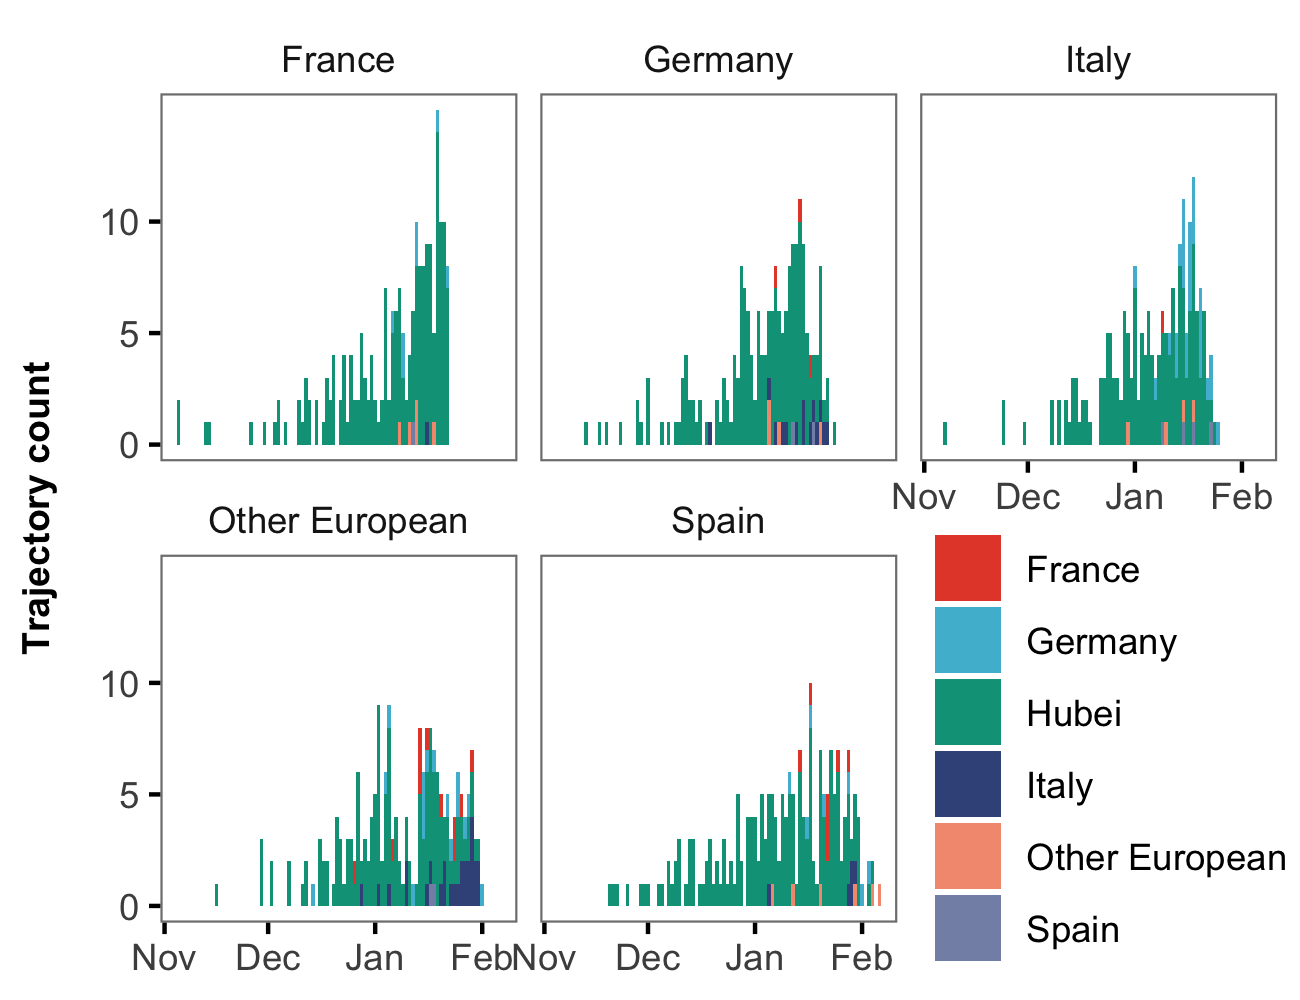
\includegraphics[width=0.5\textwidth]{201014_europe2_figtraj04.png}\label{fig:f2}}
  \caption{First introductions event time and source in each deme. (a) Distribution of the time of the first introduction for each deme from the subsampled set of trajectories. Each box and color represent one deme and the X is the first date when cases where reported to ECDC. In the case of Hubei, the distribution of the time of the origin is plotted, since it was defined as the origin of the epidemic in the analysis with probability 1. For the other five demes, the distribution of the time of the first migration into the corresponding deme is plotted. (b) Histogram of the source of the first introduction event in each deme for the set of subsampled trajectories.}
\end{figure}

\end{document}